\providecommand{\main}{../../..}
\documentclass[\main/main.tex]{subfiles}
\begin{document}

\subsection{Esercizio 5}
Dato un problema di decisione con alternative $X = \{a_1, \ldots , a_5\}$ e scenari $\Omega = \{\omega_1, \omega_2, \omega_3\}$, e con le utilità $u (f (x, \omega))$ e le probabilità $\pi (\omega)$ riportate nella tabella seguente:


\begin{table}
	\begin{tabular}{|L|L|L|L|L|L||L|}
		\hline
		u (f (x, \omega)) & a_1 & a_2 & a_3 & a_4 & a_5 & \pi (\omega) \\
		\hline
		u_1               & 80  & 100 & 50  & 0   & 90  & 0.5          \\
		\hline
		u_2               & 20  & 10  & 50  & 30  & 30  & 0.4          \\
		\hline
		u_3               & 40  & 10  & 50  & 100 & 20  & 0.1          \\
		\hline
	\end{tabular}
\end{table}

\begin{enumerate}[a)]
	\item Si elenchino le eventuali alternative dominate, specificando da quali altre alternative sono dominate.
	\item Si indichi l'alternativa scelta con il criterio del caso medio, spiegando il procedimento.
	\item Si mostri come cambia l'alternativa scelta al variare della probabilità $\pi (\omega_1)$ del primo scenario, ipotizzando che le altre mantengano le reciproche proporzioni.
\end{enumerate}

\subsection{Risoluzione esercizio 5}
\subsubsection*{Alternative dominate}
Senza considerare criteri particolari, nessuna alternativa risulta dominata.

\subsubsection*{Criterio del caso medio}
Procedendo con il criterio del caso medio, sommando le utilità pesandole con la probabilità dello scenario, si ottiene:
\begin{table}
	\begin{tabular}{|L|L|L|L|L|L|}
		\hline
		    & a_1 & a_2 & a_3 & a_4 & a_5 \\
		\hline
		u_m & 52  & 55  & 50  & 22  & 59  \\
		\hline
	\end{tabular}
\end{table}

Da cui la scelta preferibile risulta essere $a_5$.

\subsubsection*{Analisi di sensitività}
Al variare della probabilità $\pi(\omega_1)$, se le altre probabilità mantengono le stesse proporzioni, vale il sistema:

\[
	\begin{cases}
		\pi(\omega_1) = \alpha         \\
		\pi(\omega_2) = (1-\alpha)*0.8 \\
		\pi(\omega_3) = (1-\alpha)*0.2
	\end{cases}
\]

Per $\alpha\lesssim0.36$ viene scelta $a_3$, per $\alpha\gtrsim0.36\land\alpha\lesssim0.64$ viene scelta $a_5$ e per $\alpha\gtrsim0.64$ viene scelta $a_2$.

\begin{figure}
	\begin{subfigure}{0.49\textwidth}
		\begin{tikzpicture}
			\begin{axis}[
					width= \textwidth,
					xlabel=$f$,
					samples=1000,
					ylabel=$u_H$,
					domain=0:1,
					xtick = {0,0.1,0.2,...,1},
					legend style={at={(0,1)},anchor=north west}
				]
				\addplot[mark=none,color=blue]{
					100*x+10*(1-x)*0.8+10*(1-x)*0.2>=90*x+30*(1-x)*0.8+20*(1-x)*0.2?
					100*x+10*(1-x)*0.8+10*(1-x)*0.2:NaN
				};
				\addplot[mark=none,color=green]{
					50*x+50*(1-x)*0.8+50*(1-x)*0.2>=90*x+30*(1-x)*0.8+20*(1-x)*0.2?
					50*x+50*(1-x)*0.8+50*(1-x)*0.2:NaN
				};
				\addplot[mark=none]{
					50*x+50*(1-x)*0.8+50*(1-x)*0.2<=90*x+30*(1-x)*0.8+20*(1-x)*0.2&&
					100*x+10*(1-x)*0.8+10*(1-x)*0.2<=90*x+30*(1-x)*0.8+20*(1-x)*0.2?
					90*x+30*(1-x)*0.8+20*(1-x)*0.2:NaN
				};
				\legend{$a_2$,$a_3$,$a_5$}
			\end{axis}
		\end{tikzpicture}
		\caption{La massima utilità al variare della probabilità}
	\end{subfigure}
	\begin{subfigure}{0.49\textwidth}
		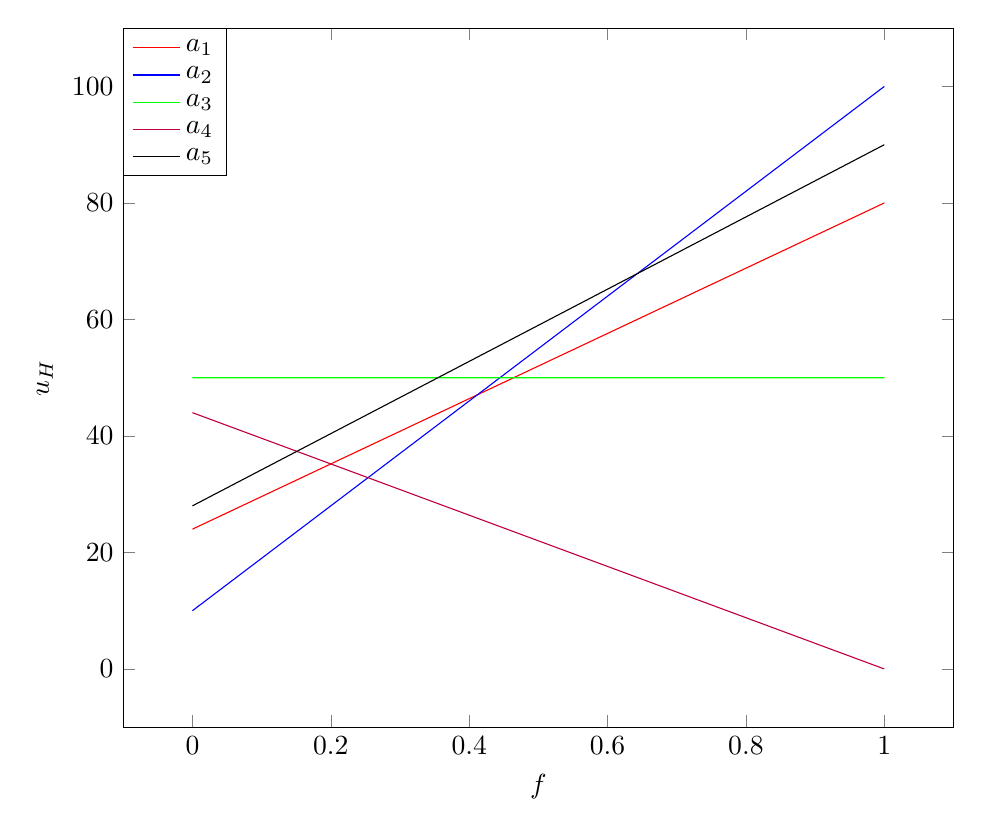
\begin{tikzpicture}
			\begin{axis}[
					width= \textwidth,
					xlabel=$f$,
					ylabel=$u_H$,
					domain=0:1,
					legend style={at={(0,1)},anchor=north west}
				]
				\addplot[mark=none,color=red]{80*x+20*(1-x)*0.8+40*(1-x)*0.2};
				\addplot[mark=none,color=blue]{100*x+10*(1-x)*0.8+10*(1-x)*0.2};
				\addplot[mark=none,color=green]{50*x+50*(1-x)*0.8+50*(1-x)*0.2};
				\addplot[mark=none,color=purple]{30*(1-x)*0.8+100*(1-x)*0.2};
				\addplot[mark=none]{90*x+30*(1-x)*0.8+20*(1-x)*0.2};
				\legend{$a_1$,$a_2$,$a_3$,$a_4$,$a_5$}
			\end{axis}
		\end{tikzpicture}
		\caption{L'utilità $u_m$ al variare della probabilità $\pi(\omega_1)$}
	\end{subfigure}
	\caption{Analisi di sensitività}
\end{figure}

\end{document}
